
%%%%%%%%%%%%%%%%%%%%%%% file typeinst.tex %%%%%%%%%%%%%%%%%%%%%%%%%
%
% This is the LaTeX source for the instructions to authors using
% the LaTeX document class 'llncs.cls' for contributions to
% the Lecture Notes in Computer Sciences series.
% http://www.springer.com/lncs       Springer Heidelberg 2006/05/04
%
% It may be used as a template for your own input - copy it
% to a new file with a new name and use it as the basis
% for your article.
%
% NB: the document class 'llncs' has its own and detailed documentation, see
% ftp://ftp.springer.de/data/pubftp/pub/tex/latex/llncs/latex2e/llncsdoc.pdf
%
%%%%%%%%%%%%%%%%%%%%%%%%%%%%%%%%%%%%%%%%%%%%%%%%%%%%%%%%%%%%%%%%%%%


\documentclass[runningheads,a4paper]{llncs}

\usepackage{amssymb}
\setcounter{tocdepth}{3}
\usepackage{graphicx}
\usepackage{subfigure}
\graphicspath{{./figure/}}
\usepackage{url}

\usepackage[ruled,lined]{algorithm2e}

\begin{document}

\mainmatter  % start of an individual contribution

% first the title is needed
\title{News Topic Evolution Tracking by Incorporating Temporal Information}

% a short form should be given in case it is too long for the running head
\titlerunning{News Topic Evolution Tracking by Incorporating Temporal Information}

% the name(s) of the author(s) follow(s) next
%
% NB: Chinese authors should write their first names(s) in front of
% their surnames. This ensures that the names appear correctly in
% the running heads and the author index.
%

\author{Jian Wang\and Xianhui Liu%
\thanks{Author to whom all correspondence should be addressed; e-mail: lxh@tongji.edu.cn}%
\and Junli Wang\and Weidong Zhao}

\authorrunning{Jian Wang}
% (feature abused for this document to repeat the title also on left hand pages)

% the affiliations are given next; don't give your e-mail address
% unless you accept that it will be published

\institute{Engineering Research Centre of Ministry of Education \\
on Enterprise Digitalization Technology, Tongji University, China}

%
% NB: a more complex sample for affiliations and the mapping to the
% corresponding authors can be found in the file "llncs.dem"
% (search for the string "\mainmatter" where a contribution starts).
% "llncs.dem" accompanies the document class "llncs.cls".
%

\maketitle


\begin{abstract}
Time stamped texts or text sequences are ubiquitous in real life, such as news reports. Tracking the topic evolution of these texts has been an issue of considerable interest. Recent work has developed methods of tracking topic shifting over long time scales. However, most of these researches focus on a large corpus. Also, they only focus on the text itself and no attempt have been made to explore the temporal distribution of the corpus, which could provide meaningful and comprehensive clues for topic tracking. In this paper, we formally address this problem and put forward a novel method based on the topic model. We investigate the temporal distribution of news reports of a specific event and try to integrate this information with a topic model to enhance the performance of topic model. By focusing on a specific news event, we try to reveal more details about the event, such as, how many stages are there in the event, what aspect does each stage focus on, etc.
\keywords{Temporal Distribution, LDA, News Topic Evolution}
\end{abstract}


%% *** BEGINNING OF MAIN TEXT ***
\section{Introduction}
\label{Introduction}
Online news spreads across the Internet due to its features of responsiveness and customization. Information with regard to the events occurring around the world can be known quickly via these channels. People may keep track of the development of the news topic for individual or institutional interest. However, with the dramatic increase of these digital document collections, the amount of information is far more beyond that person can efficiently and effectively process. There is a great demand for developing automatic text analysis models for analyzing these collections and organizing its contents. Probabilistic topic models, such as Latent Dirichlet Allocation (LDA) \cite{Blei:2003}, Author-Topic Model \cite{rosen2004author} were proven to be very useful tools to address these issues.

To face the continuously evolving news events, topic detection and tracking (TDT) \cite{allan2002introduction} techniques have been developed to divide news reports into groups and keep track of future events corresponding to the topic. Mechanisms developed in TDT research enable news readers to identify clustered news collections. But it is still cognitive and time consuming for readers who want to comprehend the evolution of the news topic. With the need to model the time evolution of topics in large document collections, a family of probabilistic time series models were developed. Dynamic topic model (DTM) \cite{Blei:2006} captures the evolution of topics in a sequentially organized corpus of documents. DTM divides documents into several time slices, and in each episode, LDA is applied to explore the topic distribution. While time is intrinsically continuous, discretization of time always face the question of selecting the slice size, and the size is inevitably too small for some regions and too large for others. Topic over Time (TOT) \cite{wang2006topics} model treats time as a continuous variable. Continuous Dynamic Topic Model (cDTM) \cite{wang2008continuous} uses Brownian motion to model continuous time topic evolution. iDTM \cite{ahmed2012timeline} is an infinite dynamic topic model which allows for an unbounded number of topics and captures the appearance and vanishing of topics.

These models are quite useful when dealing with corpus with many different topics mixed up, but when it comes to a specific news event, the result seems to be not such remarkable. A couple of methods for generating timeline were proposed to deal with these issues in recent year \cite{tang2013discovery} \cite{zehnalova2012evolution} \cite{lin2012generating}.  \cite{wang2009evolutionary} develops an evolutionary document summarization system for discovering the changes and differences in each phase of a disaster evolution. \cite{berendt2009stories} presents the STORIES methods and tool for learning an abstracted story representation from a collection of time-indexed documents. \cite{wang2012generating} introduces a novel framework for generating pictorial story lines for the given topics from text and image data.

However, most of these methods are trying to get a summarization of the event from the text but none of these methods mentioned above have taken the advantage of the temporal information as a prior knowledge. In this paper, we first explore the temporal distribution of news event, then propose an algorithm to automatically divide the corpus into different stages, in which the documents may have more coherence. By incorporating temporal information to topic model, we introduce a framework for tracking a specific news event evolution. The rest of this paper is organized as follows. In section 2, we discuss some background knowledge used in this paper. In section 3, we illustrate the temporal distribution of the news event and describe the division algorithm in detail. In section 4, we propose our analysis framework and explain how temporal information can enhance the topic model. In section 5, we present the case study experiment in detail. In section 6, we conclude the paper with some analysis and outlook for future work.

\section{Background Knowledge}
\label{background knowledge}
In this section, we lay the foundation for the rest of this paper by introducing some relevant and detailed background knowledge.
\subsection{Topic model}
\label{topic model}
Topic Model like LDA \cite{Blei:2003}  is a probabilistic generative model that can be used to estimate the properties of multinomial observations by unsupervised learning. In topic model, an article is assumed to contain multiple topics, thus a document is viewed as a probability distribution over topics, and each topic is treated as a distribution over words. If we have $K$ topics, we can write the probability of the $i$th word in a given document as
\begin{equation}
P(w_i)=\sum_{j=1}^{K}P(w_i|z_i=j)P(z_i=j)
\end{equation}
where $z_i$ is a latent variable indicating the topic from which the $i$th word was drawn and $P(w_i|z_i=j)$ is the probability of the word $w_i$ under the $j$th topic. $P(z_i=j)$ gives the probability of choosing a word from topics $j$ in the current document, which will vary across different documents.  Let $\vec{\varphi}_k$ denotes the multinomial distribution of topic $k$ over a $V$-word vocabulary, $\vec{\vartheta}_m$ denotes the multinomial distribution of document $m$ over $K$ topics. LDA model describe the generate process of the corpus with $M$ documents as follow:
\begin{enumerate}
  \item sample mixture component $\vec{\varphi}_k \sim Dir(\vec{\beta})$ for all topics $k \in [1, K]$
  \item for all documents $m \in [i, M]$ 
  \begin{enumerate}
    \item sample mixture proportion $\vec{\vartheta}_m \sim Dir(\vec{\alpha})$
    \item sample document length $N_m \sim Poiss(\xi)$
    \item for all words $n \in [1, N_m]$
    \begin{enumerate}
      \item sample topic index $z_{m,n} \sim Mult(\vec{\vartheta})$
      \item sample term for word $w_{m,n} \sim Mult(\vec{\varphi}_{z_{m,n}})$
    \end{enumerate}
  \end{enumerate}
\end{enumerate}
where $Dir(\cdot)$ denotes the Dirichlet Distribution, $\vec{\alpha}$ is a $K$-dimensional vector, $\vec{\beta}$ is a $V$-dimensional vector; $Mult(\cdot)$ denotes the multinomial distribution, $Possi(\cdot)$ denotes the Poisson distribution. 

Although LDA is still a relatively simple model, exact inference is generally intractable. The solution to this is to use Approximate inference algorithms, such as Gibbs sampling\cite{griffiths2004finding}.

\subsection{Gibbs Sampling}
\label{gibbs sampling}
Gibbs sampling is a special case of Markov Chain Monte Carlo (MCMC) simulation \cite{mackay2003information} and often yields relatively simple algorithms for approximate inference in high-dimensional models. MCMC methods can emulate high-dimensional probability distribution $p(\vec{x})$ by the stationary behavior of a Markov chain. This means that one sample is generated for each transition in the chain after a stationary state of the chain has been reached, which happens after a so-called "burn-in period" that eliminates the influence of initialization parameters\cite{Walsh:2004}. Gibbs sampling is special case of MCMC where the dimension $x_i$ of the distribution are sampled alternately one at a time, conditioned on the values of all other dimensions.

The target of inference is the distribution $p(\vec{z}|\vec{w})$, which is directly proportional to the joint distribution. The $z_{m,n}$ denotes the topic for the word n in document m.
\begin{equation}
p(\vec{z}|\vec{w})=\frac{p(\vec{z}, \vec{w})}{p(\vec{w})} \propto p(\vec{z}, \vec{w}) = p(\vec{z}, \vec{w}|\vec{\alpha},\vec{\beta}) = p(\vec{w}|\vec{z},\vec{\beta})p(\vec{z}|\vec{\alpha})
\end{equation}
Because the multinomial distribution is conjugate to Dirichlet distribution, so the $\varphi_k$ and the $\vartheta_m$ can be integrated out. From the joint distribution we can derive the full conditional distribution for a word token $p(z_i=k|\vec{z}_{\neg i},\vec{w})$ with index $i=(m,n)$. With all the value of $\vec{z}$ inferred, we can using the expectation of the Dirichlet distribution to yield(more details can be found in\cite{heinrich2005parameter}):
\begin{equation}
\varphi_{k,t}=\frac{n_{k}^{t}+\beta_{t}}{\sum_{t=1}^{V}n_{k}^{t} \; +\beta_{t}}
\end{equation} 
\begin{equation}
\vartheta_{m,k}=\frac{n_{m}^{k}+\alpha_k}{\sum_{k=1}^{K}n_{m}^{k} \; +\alpha_k}
\end{equation} 

\section{Temporal Distribution of News Events}
\label{temporal distribution of news events}
When a sensational event burst out, all the newspapers would immediately report it. So, in a sudden time, related reports will overflow in media. Later the quantity of related reports would gradually decline for many reasons. But once new details are disclosed or someone else is involved, the event gains its popularity again and likewise the amount of related reports would move up sharply. Suppose we label each of the popular period as a stage. Generally, most news events may have several stages, and each stage has its own focus. Between the two adjacent stages, there would be less related reports found on the news websites. The results showed in the Fig.\ref{temporal distribution} are exactly in conformity with what we've assumed above. 
% figure — temporal distribution of news reports quantity
\begin{figure}[htb]
	\subfigure[Edward Snowden]{
		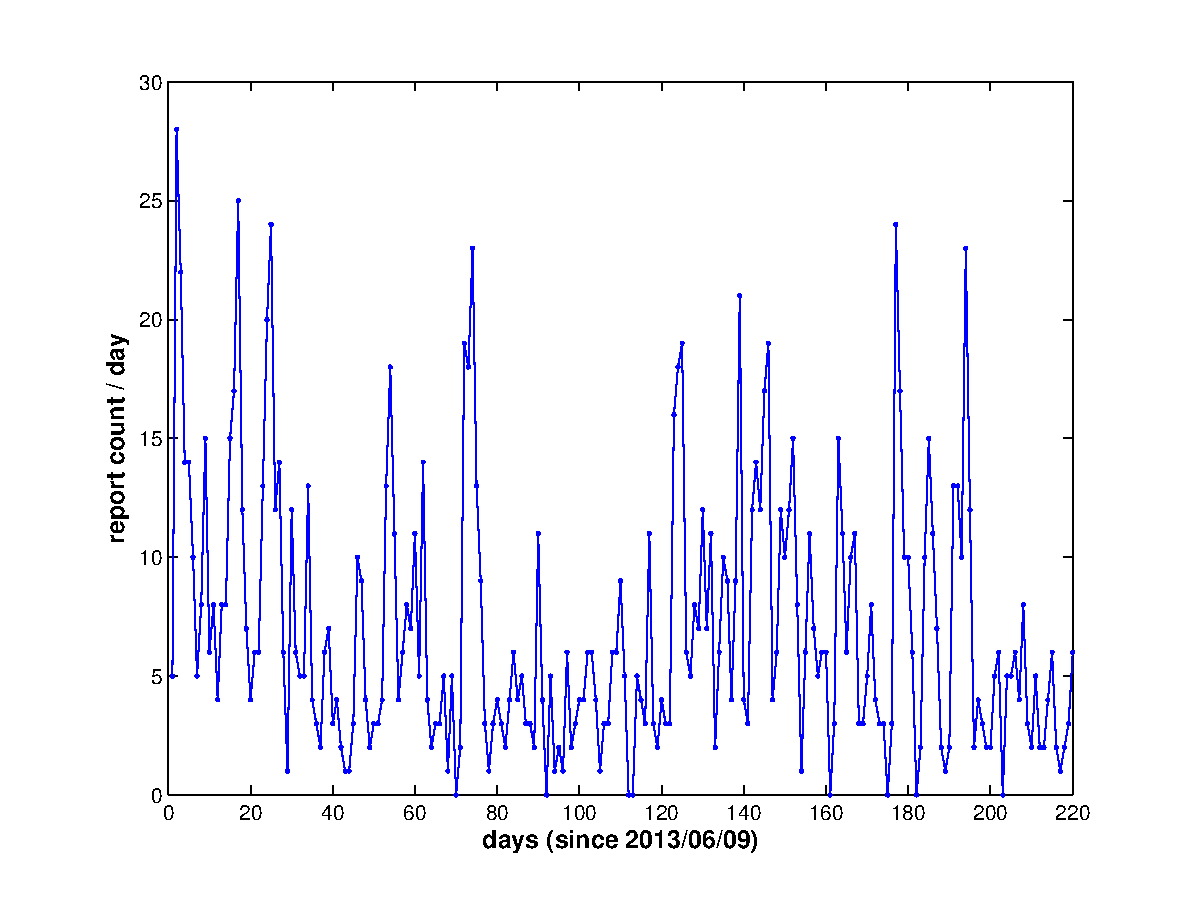
\includegraphics[width=5.8cm]{guardian_snowden}
		\label{temporal distribution:snowden}
	}
	\subfigure[Obamacare]{
		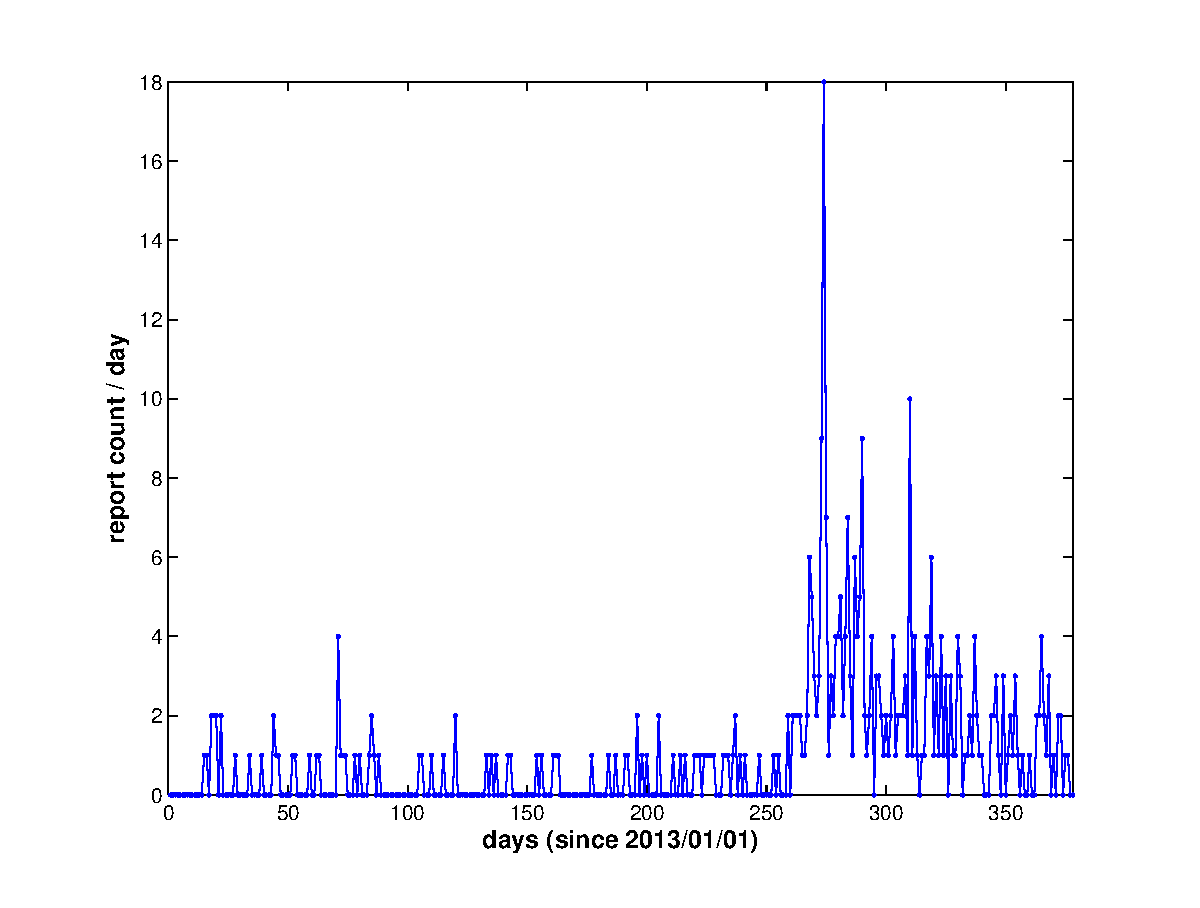
\includegraphics[width=5.8cm]{guardian_obamacare}
		\label{temporal distribution:obamacare}
	}
	\caption{Temporal distribution of news reports quantity about "Edward Snowden" and "Obamacare". X-axis represents day's interval from the beginning date and the Y-axis represents article count. Articles were crawled from The Guardian with the key words "Edward Snowden" from 9 June 2013 to 10 Jan 2014, and "Obamacare" from 1 Jan 2013 to 10 Jan 2014.}
	\label{temporal distribution}
\end{figure}

\subsection{Documents Division and the Adaptive K-Means algorithm}
\label{news documents division}
We've been thinking over that whether it would enhance the performance of topic model while analyzing the evolution of a specific news topic by incorporating temporal distribution information. In Blei's DTM \cite{Blei:2006}, the corpus was evenly divided by time, thus every episode has the same time scale. Let's take a look at the Fig.1, if the documents are divided by time evenly, the dividing points may just locate at the peak point. Intuitively, this is not a good choice. Because the reports around the peak point mainly focus on the same aspect and they have a strong coherence.

From the analysis above, we've gain some knowledge about what is a good division of documents. So next, we propose a simple but efficient method which is called the Adaptive K-Means algorithm. This algorithm is based on the K-Means algorithm\cite{kanungo2002efficient} and could automatically divide the documents without setting the cluster number K in advance. In this paper the cluster number K means the episode number. But we have no idea how many episodes could best suit the corpus. With the Adaptive K-Means algorithm, the best number of K is automatically decided. The corpus is then divided into K subsets with different time span and article count. The algorithm is described as follow:

% pseudocode adaptive k-means algorithm
\begin{algorithm}
  \DontPrintSemicolon
  \KwData{$X$: news count of each day; $max\_k$: the maximum value of K; $t$: threshold value}
  \KwResult{$count$: article count of each episode; $dists$: weighted mean distance array; $K$: the best count of cluster}
  \BlankLine
  $Y \longleftarrow$ remove $zero$ points from $X$\;
  \For{$i \leftarrow 1$ \KwTo $max\_k$}{
    $[count, sumd]=kmeans(Y, i)$;\;
    \tcp*[r]{$count$: point count of each cluster}
    \tcp*[r]{$sumd$: sum distance of each cluster}
    $means \leftarrow calc\_mean\_distance(count, sumd)$;\;
    \tcp*[r]{$means$: mean distances of all clusters}
    $dists[i] \leftarrow calc\_weighted\_mean\_distance(means)$;\; 
    \If{$i > 1$} {
      \If{$dists[i]-dists[i-1] < t$}{
        $K \leftarrow (i-1)$; break;
      }
    }
  }
  \If{$K = 0$} {$K \leftarrow max\_k$;\;}
  \caption{Adaptive K-Means algorithm}
  \label{algorithm1}
\end{algorithm}

The Adaptive K-Means algorithm starts with a small number of clusters, and adds the number one by one. At each iteration of the algorithm, we calculate the \emph{weighted mean distance} of all clusters. The \emph{weighted mean distance} is defined as follows:
\begin{equation}\label{eq:wmd}
Weighted\;Mean\;Distance=\frac{\sum_{i=1}^{n}{mean\;distance\;of\;cluster\;i}}{n}
\end{equation}
The distance calculated in the Equation.\ref{eq:wmd} refers to Euclidean distance. In the beginning, the number of centers is much smaller than the best $K$, so the \emph{Weighted Mean Distance} would decline rapidly. With the number getting closer to the best $K$, the decrease value becomes smaller and smaller. Once the decrease value is smaller than a specific threshold value, then the current number of centers is regarded as the best $K$.

\section{Incorporating Temporal Information into Topic Model}
\label{section4}
In this section, we illustrate how to use topic model to track news topic evolution and why temporal information can improve the analysis result.

\subsection{Basic Concepts}
\label{section4.1}
First of all, we would like to give the explicit definitions of some basic concepts which would be frequently mentioned. A \textbf{\emph{stage}} is a time episode in which documents have a strong coherence, and documents are likely related to a same aspect of the event. Stages exhibit some common characters:
\begin{enumerate}
	\item Within a stage, all documents have a strong coherence;
	\item Stage $i$ evolves from stage $i$-1, they both hold a same \textbf{\emph{main topic}} which could run throughout all stages; the main topic is the line connecting all the episodes and varies little along the time;
	\item Except for the main topic, all the other topics are called the \textbf{\emph{auxiliary topics}}, which present the new aspects of the main topic in different stages; The auxiliary topics could be regarded as the progresses of the event because they very a lot along the time
\end{enumerate}

\subsection{Framework of Our Method}
\label{section4.2}
Our analytical framework is based on the LDA \cite{Blei:2003}, a generative latent variable model that treats documents as bags of words generated by one or more topics. Each document is characterized by a multinomial distribution over topics, and each topic is in turn characterized by a multinomial distribution over words. We perform parameter estimation using collapsed Gibbs sampling \cite{griffiths2004finding} \cite{heinrich2005parameter}. Since LDA assumes that all documents in the corpus are exchangeable, it does not apply to corpus which has an apparent character of time sequence, like news documents. However, we could firstly divide the corpus into several subsets by time, and apply LDA within each subset, respectively. As for the division, we've described the \emph{Adaptive K-Means algorithm} above which makes more sense than the method of simply dividing the corpus by time evenly

By incorporating temporal information, the overall framework of analysis process is as follows:
\begin{enumerate}
  \item Prepare documents for each episode with \emph{Adaptive K-Means algorithm};
  \item Preprocess of the documents in each episode;
  \item Draw topic distribution of each episode from topic model (LDA);
  \item Discover the main topic and draw the evolution map of the event.
\end{enumerate}

\subsection{Main Topic Discovery}
\label{section4.3}
As is defined above, the main topic is the one which has the most similarities between two adjacent episodes. In order to discover the main topic and track the evolution, we need to calculate the similarity between adjacent episodes. As the topic is characterized by a distribution over words. A simple measure method of similarity between topics is the \emph{Kullback-Leibler divergence} (also called \emph{relative entropy}). For discrete probability distribution $P$ and $Q$, the \emph{KL divergence} is defined to be
\begin{equation}
D_{KL} \left ( P||Q \right ) = \sum_{i}ln\left ( \frac{P(i)}{Q(i)} \right ) P(i)
\end{equation}
However, the \emph{KL divergence} is not a proper distance measure method because it is not symmetric. An alternative option is the \emph{Jensen-Shannon distance}, which is a smoothed and symmetric extension of the \emph{KL divergence}.
\begin{equation}
D_{JS} \left ( P||Q \right ) = \frac{1}{2} D_{KL} \left ( P||M \right ) + \frac{1}{2} D_{KL} \left ( Q||M \right )
\end{equation}
With the averaged variable $M = \frac{1}{2}(P+Q)$. 

\subsection{Document Coherence and Evaluation}
\label{section4.4}
\emph{Document Coherence} measures the topic similarity among documents. Intuitively, if articles within a corpus are more coherent, more detail could be revealed by topic models. For example, in this paper we collected articles of two news event, there are two ways to analyse these articles. One is mixing these articles up as one corpus before applying topic models, the other is applying topic model to the two corpora, respectively. Obviously, we can learn more details about the two events from result of the latter one.

In other words, when using topic model to analyse the corpus, if the articles within a time episode have more similarities or are more coherent, the result could be more explicit and the event could be better understood.

Variance is always a good indicator while measuring the coherence of data. But in order to better present document coherence we propose a new evaluation method which is called \emph{n Topic Coverage Rate($TCR_n$)}.
\begin{equation}\label{eq:tcr}
TCR_n = \frac{\left \| articles\;\;belong\;to\;these\;n\;topics \right \|}{\left \| all\;articles \right \|} * 100\%
\end{equation}
In this equation, $\left \| \cdot \right \|$ denotes the element count of a collection. $TCR_n$ measures the documents cover rate of the top $n$ topics within the whole corpus. From the Equation.\ref{eq:tcr}, we can see that with topic number $n$ fixed, the bigger the $TCR_n$ is, the more coherent the articles are. In other words, with the $TCR_n$ fixed,  the smaller the $n$ is, the more coherent the articles are.

\section{Experiment Result and Analysis}
\label{section5}
In this section we illustrate the result of the topic model with temporal information incorporated. First of all, we demonstrate the division result of the \emph{Adaptive K-Means algorithm} with two corpora, and later focus on one of them to give a deep illustration. We analyze 1550 documents crawled from the Guardian with the key words "Edward Snowden" which is one of the top events of 2013. The time of these documents varies from June 9 of year 2013 to the end of year 2013. Our corpus is made up of approximately 1.5 million words. First of all, we use Stanford Parser\footnote{\url{http://nlp.stanford.edu/software/lex-parser.shtml}} to parse the full text, and only keep words which are noun, proper noun, verb and adjective. Next, we lemmatize the remaining words. At last, we prune the vocabulary by removing stop words and removing terms that occurred less than 5 times. The remaining vocabulary size is 7732.

\subsection{Result of the \emph{Adaptive K-Means Algorithm}}
\label{section5.1}
Since our corpora contain documents covering a period of one year, we estimate the maximum value of the episode number to be 20 in our experiments. The threshold value is 0.5. Once the decrease value of \emph{weighted mean distance} is less than the threshold and this algorithm returns, the final episode number $K$ is set to the current cluster number. Otherwise, if the cluster number is bigger than the maximum value and this algorithm also returns, the best episode number $K$ is set to the maximum value.

FigFig.\ref{cluster} shows the automatically divided result of the two event "Edward Snowden" and "Obamacare". From the result we can find each episode has a different time span which is highly corresponding to the temporal distribution information.
% figures — results of adaptive k-means algorithm
\begin{figure}[htb]
	\subfigure[Edward Snowden]{
		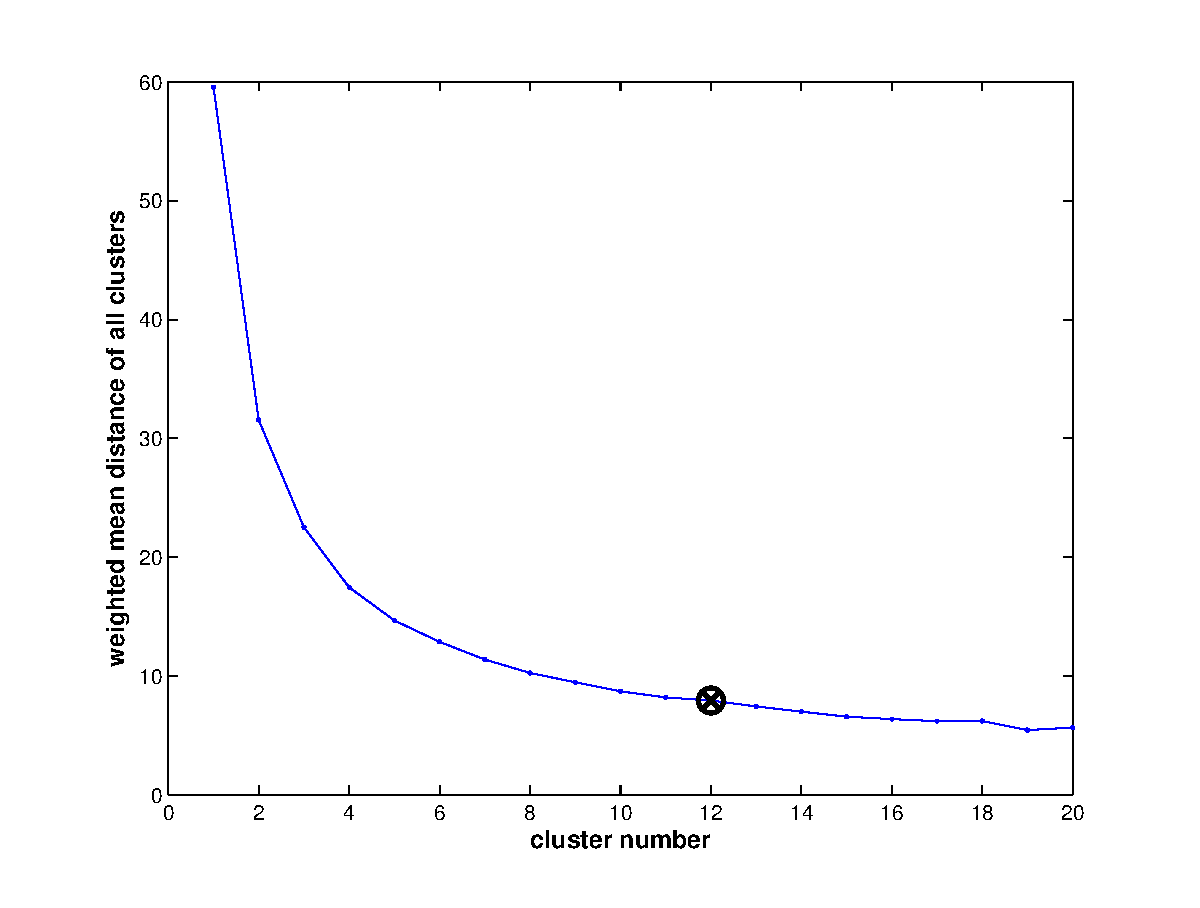
\includegraphics[width=5.8cm]{guardian_snowden_change}
		\label{cluster:snowdenTrend}
	}
	\subfigure[Edward Snowden]{
		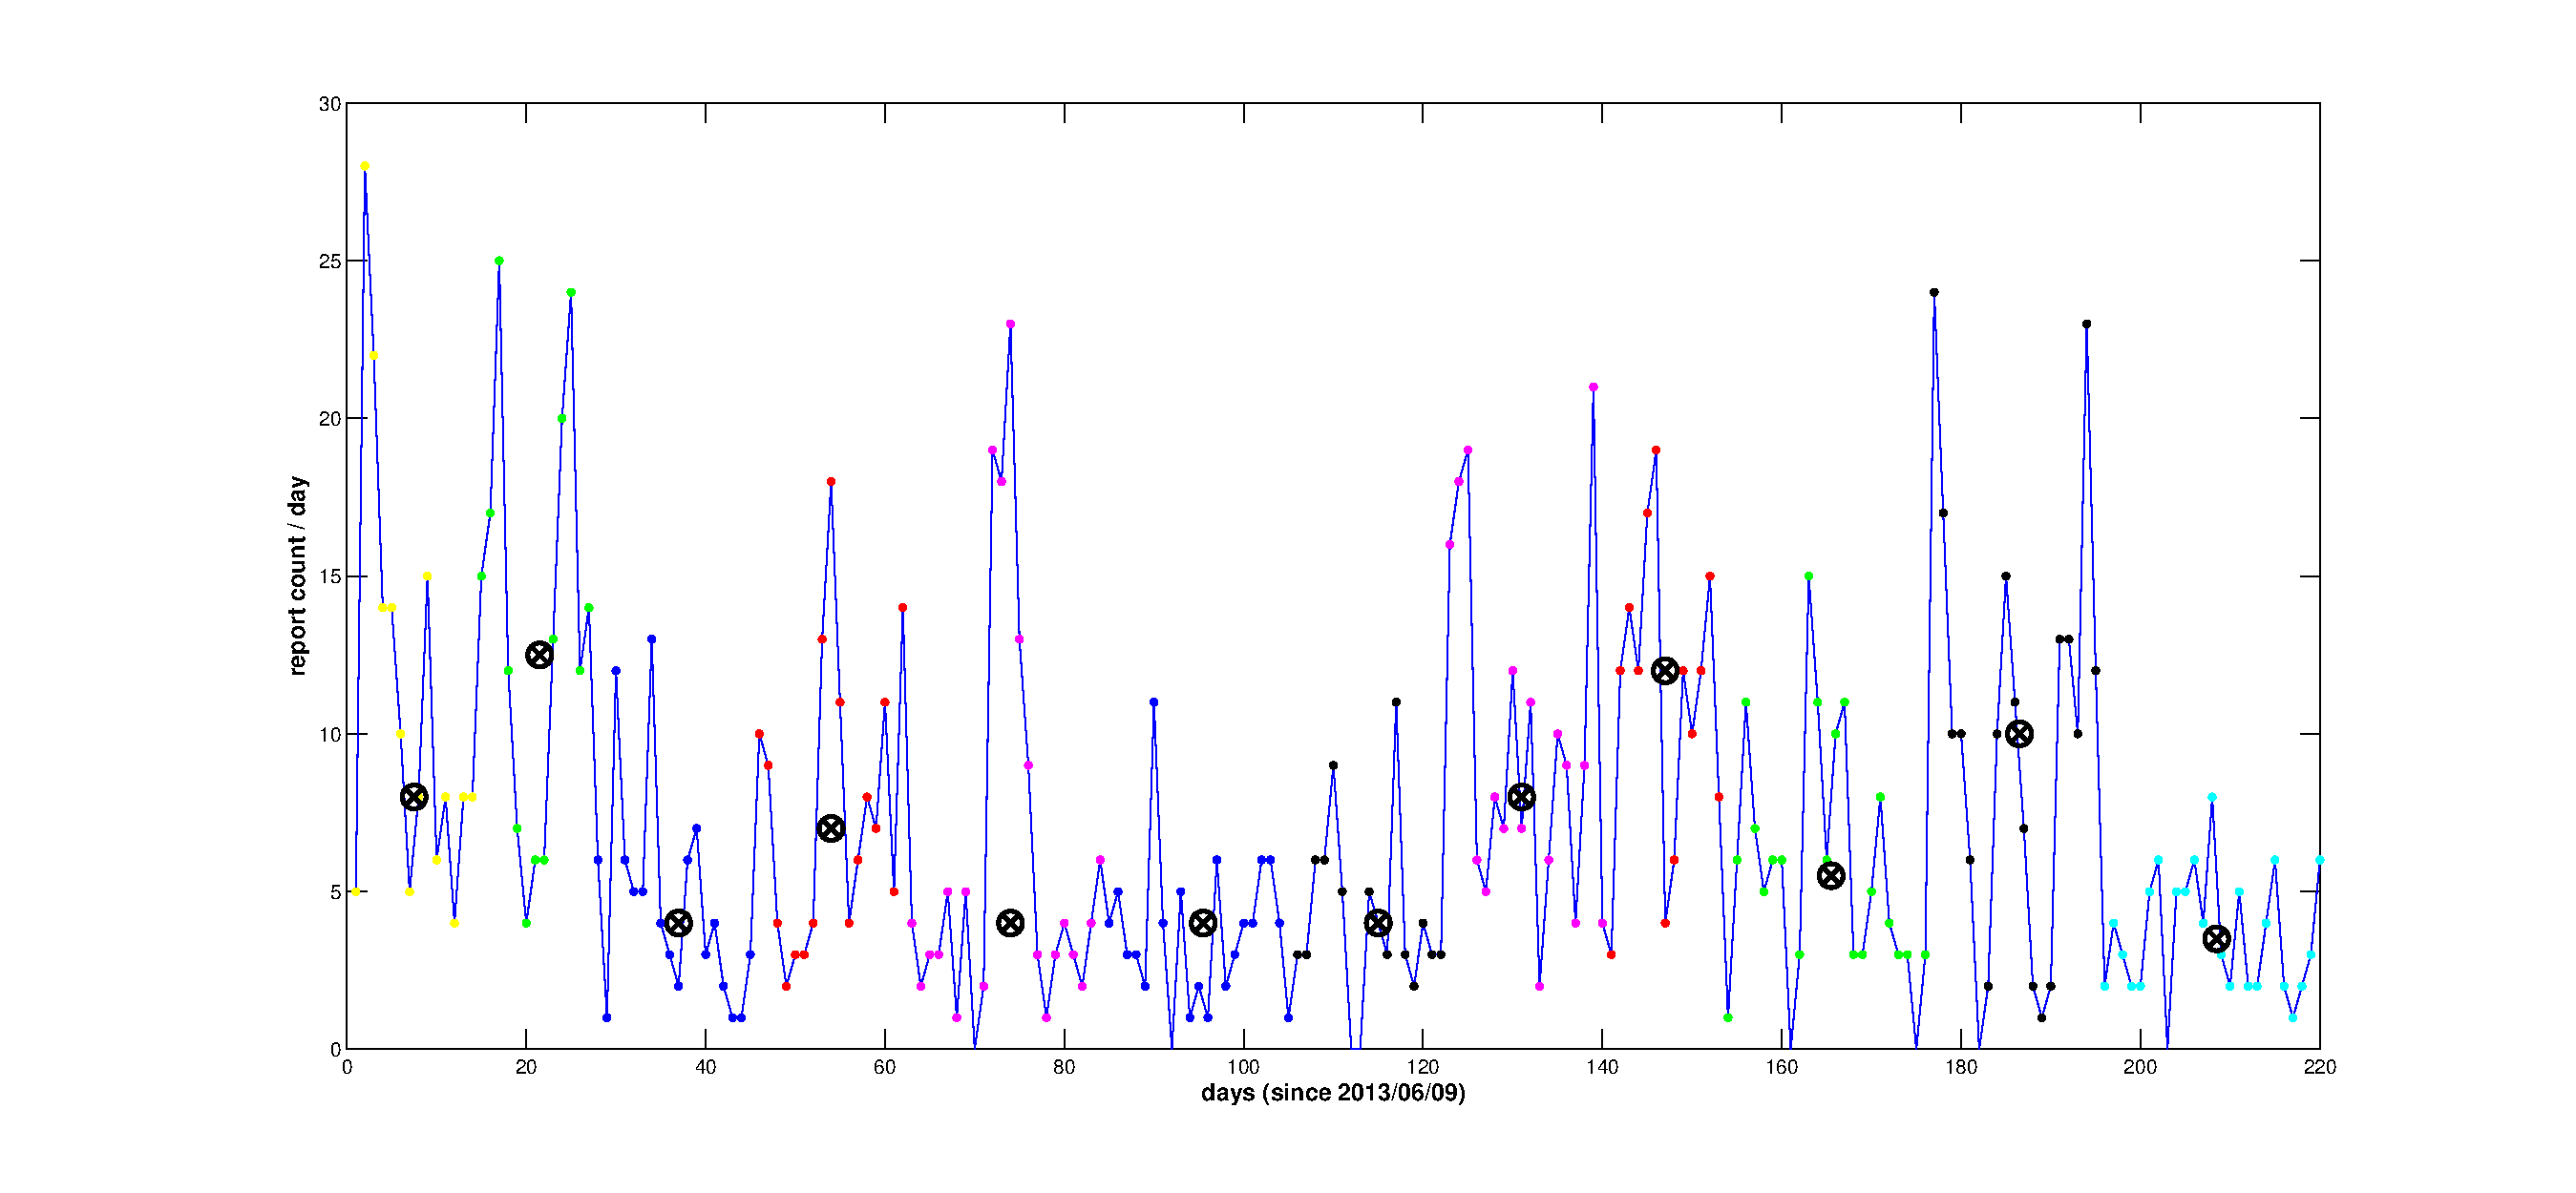
\includegraphics[width=5.8cm]{guardian_snowden_cluster}
		\label{cluster:snowdenResult}
	}
	\subfigure[Obamacare]{
		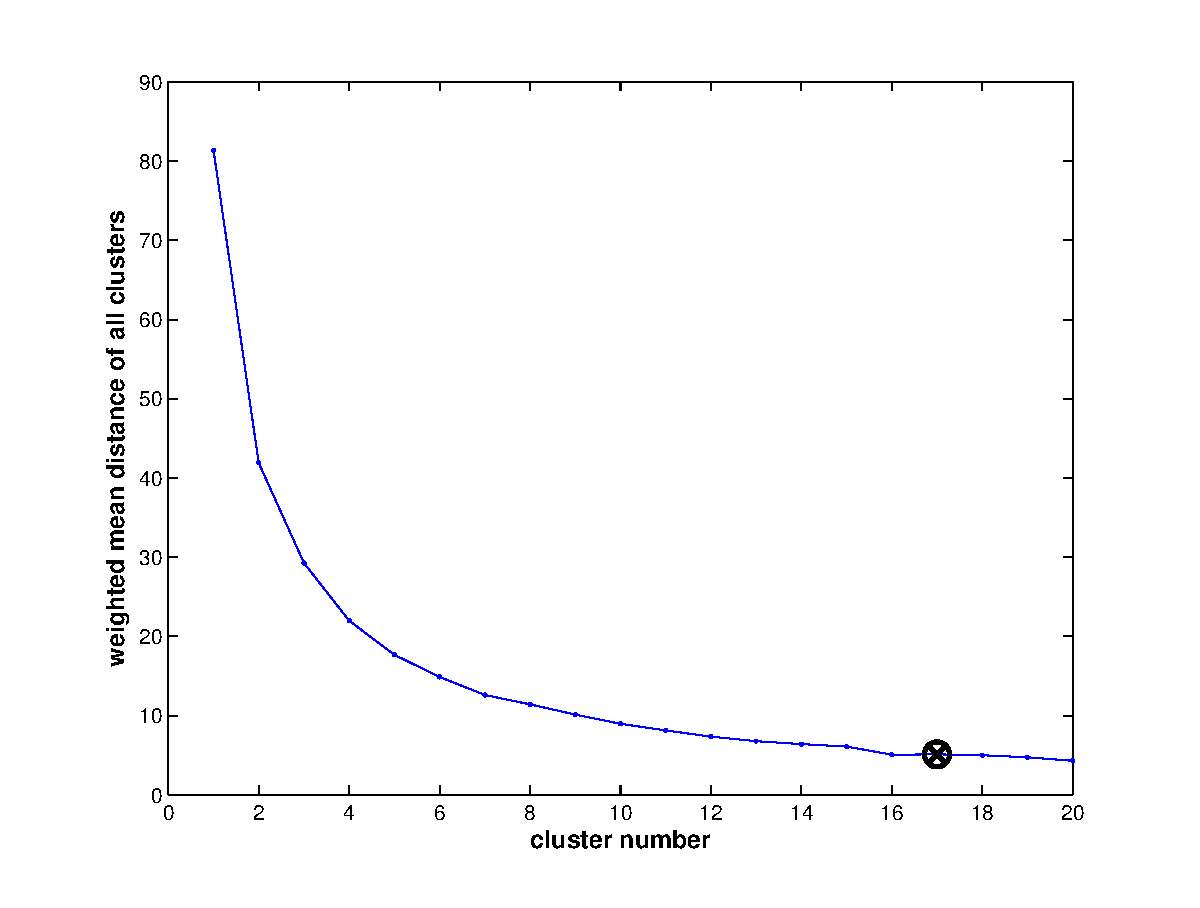
\includegraphics[width=5.8cm]{guardian_obamacare_change}
		\label{cluster:obamacareTrend}
	}
	\subfigure[Obamacare]{
		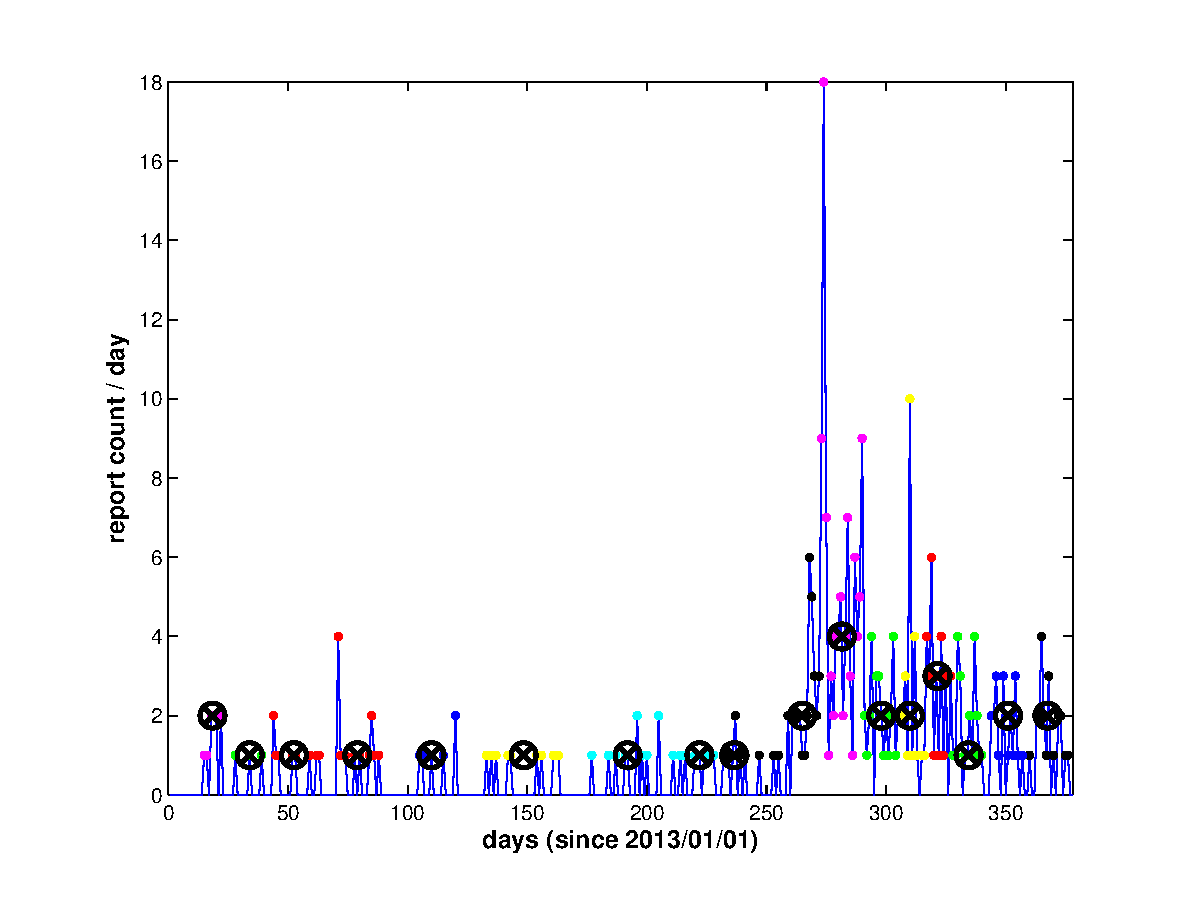
\includegraphics[width=5.8cm]{guardian_obamacare_cluster}
		\label{cluster:obamacareResult}
	}	
	\caption{Cluster number determination process and documents division results by applying adaptive K-Means algorithm. The black $\otimes$ indicates the best number of clusters in (a) (c), and the centre point in (b) (d). In (b) (d), data points in different clusters are labelled with different colours}
	\label{cluster}
\end{figure}

\subsection{Document Coherence Analysis}
\label{section5.2}
By applying the \emph{Adaptive K-Means algorithm}, our corpus of "Edward Snowden" is divided into 12 subsets. For the sake of document coherence comparison, we also divide the corpus into another 12 subsets by time evenly. We set the initialization parameters as follow: LDA parameters, $\alpha$=2 and $\beta$=0.5; Gibbs sampling parameters, total iterations=1000, burn-in iterations=200, sample intervalFig.=3. After running topic model in each episode, respectively, we calculate $TCR_n$ of all episodes. Fig.\ref{TCR5} is an example of top 5 topics' coverage. Obviously, our division algorithm has a higher coverage, which means documents in the subset have a stronger coherence. To be more convincible, we calculate the average coverage rates of all episodes with different topic numbers, and the Fig.\ref{TCR5} shows that our method has a general advantage.
\begin{figure}[htb]
	\centering
	\subfigure[$TCR_5$]{
		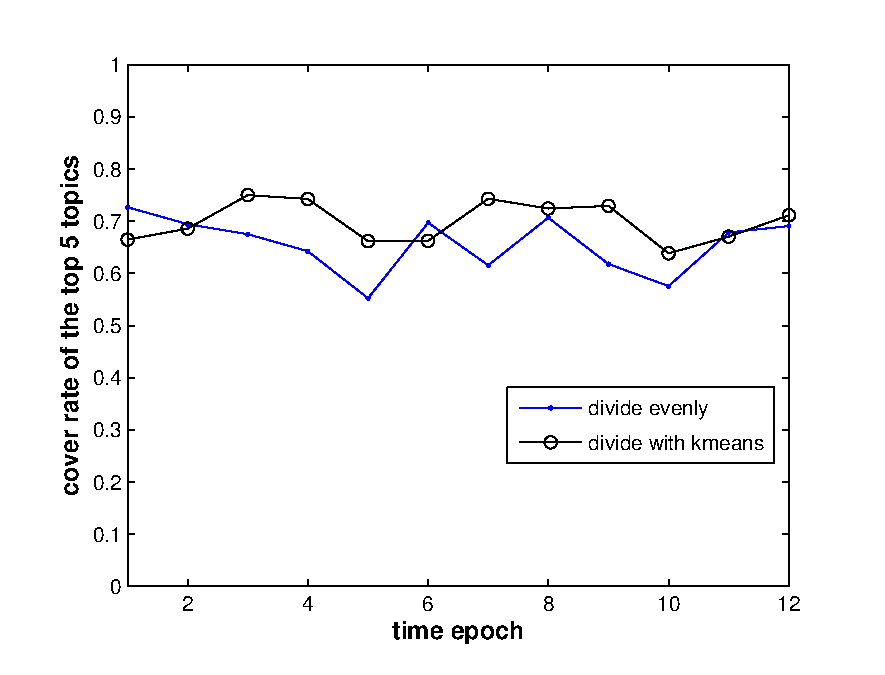
\includegraphics[width=5.8cm]{cover_rate_snowden_5_topic}
		\label{TCR5}
	}
	\subfigure[Average $TCR_n$]{
		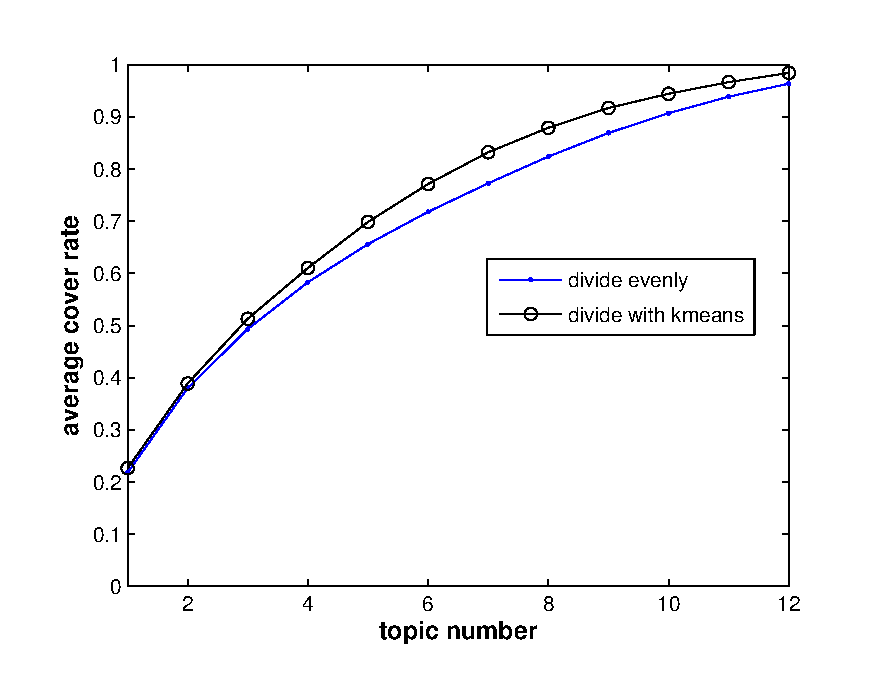
\includegraphics[width=5.8cm]{avg_cover_rate_snowden}
		\label{TCRn}
	}	
	\caption{$TCR_n$ of corpus about "Edward Snowden"}
	\label{TCR}
\end{figure}

\subsection{Evolution Map of "Edward Snowden"}
\label{section5.3}
Considering that the corpus is about one specific event and there won't be too many aspects in each episode, so we only pick the top 3 topics of each episode to draw the \textbf{evolution map}.

\begin{figure}[htb]
	\centering
	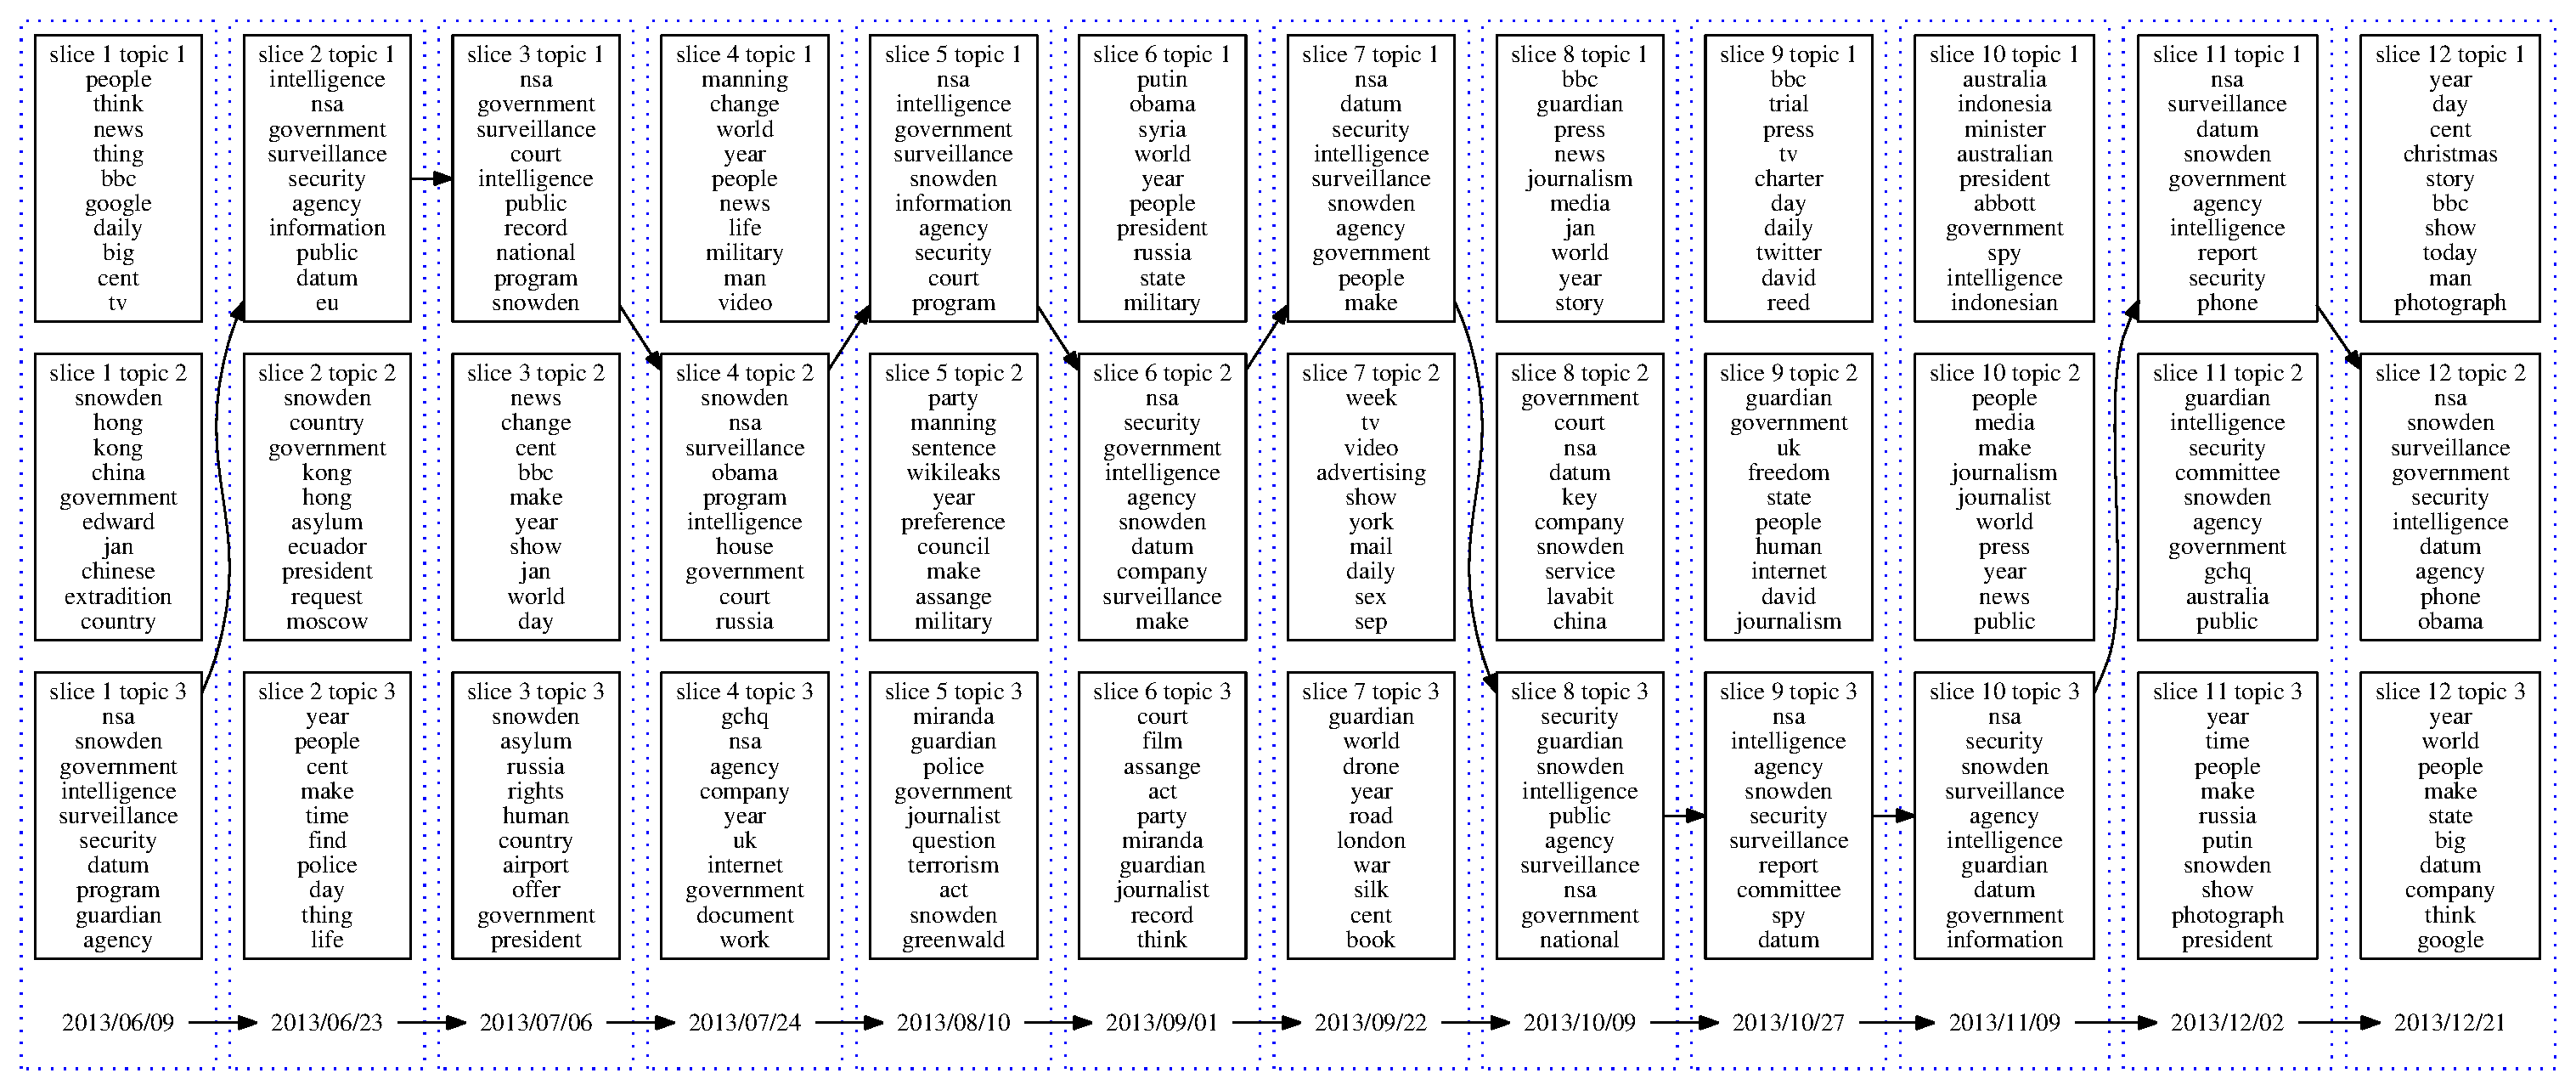
\includegraphics[width=12cm]{evolution_lda_kmeans}
	\caption{Topics evolution map of the event "Edward Snowden" by the method of this paper}
	\label{evolution:our}
\end{figure}
Fig.\ref{evolution:our} is the evolution map of the event "Edward Snowden" drawn from the method introduced in this paper. On this map, the main topic which runs throughout all stages is the one chained with arrow lines. From the main topic, we can see that the corpus is about the "\emph{Snowden leaks information about the intelligence surveillance of NSA government's security agency}". As for the first episode, we can know "\emph{Snowden comes to Hong Kong China and announces on the TV}" from the auxiliary topics. From the auxiliary topics of the second episode, we can know that "\emph{Snowden makes requests for asylums}". Also from auxiliary topics of the third episode, we can know that "\emph{Snowden stays in airport for a couple of days, and finally the Russia government offers him asylum}". In this way, we can gain an overall view of the whole progress about this event from the evolution map.

\begin{figure}[htb]
	\centering
	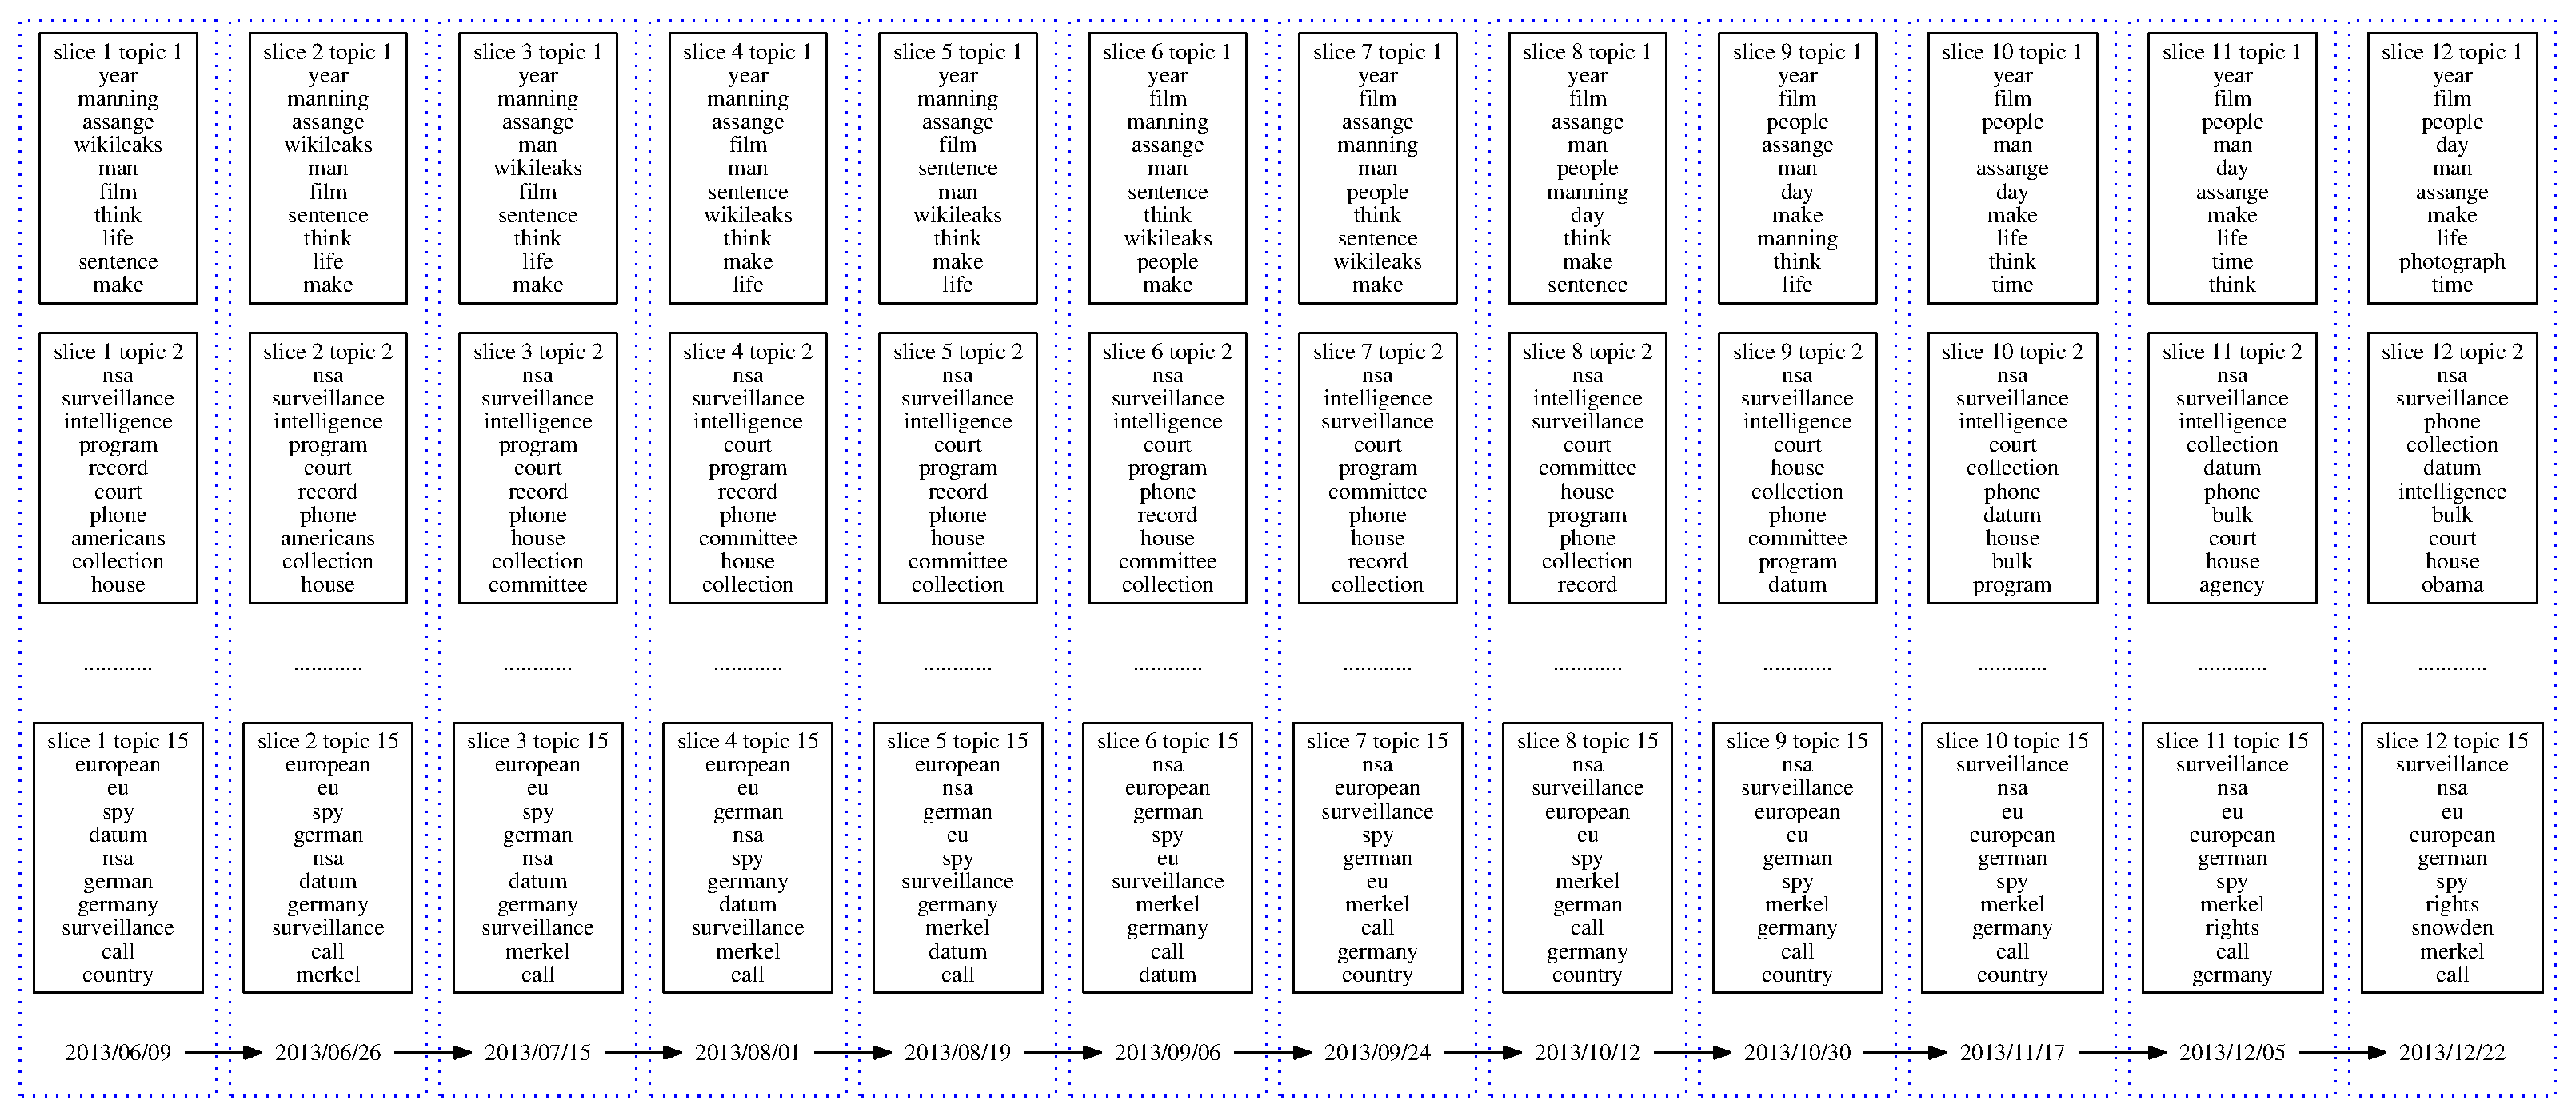
\includegraphics[width=12cm]{evolution_dtm_15}
	\caption{Topics evolution map of the event "Edward Snowden" by the DTM}
	\label{evolution:dtm}
\end{figure}
To make a contrast, we also apply the DTM to generate evolution map. DTM assumes that topic number is fixed during all episodes and no new topic would emerge and all the topics are evolved from the first episode. Thus, it is suitable for the corpus that contains many different topics, such as academic documents. While in this paper, we concentrate on a specific news event, so it is not applicable. The experiment result has also proved such point. Look at the Fig.\ref{evolution:dtm}, this is the result drawn from DTM, with 12 episodes and 15 topics in each episode (for a better view, we omit the topic 3-14 of each episode). It is very clear that topics in all the episodes seem to be almost the same. From this evolution map, we can hardly know the progresses of the event.

\section{Conclusion}
\label{conclusion}
In this paper, we address the problem of modeling sequence documents related to a specified news event. We explore the temporal distribution of news reports and treat them as a prior knowledge of the sequence topic model. To the best of our knowledge, no work has been found in combining the temporal information with topic model. By applying our method to the article collections crawled from the Guardian about "Edward Snowden", we draw an evolution map which provides an overall view of the event. Also the evolution map can be used as an input of a summarization system. In the future, we plan to model the entities involved in the event and explore how they influence the event evolution. We also intend to develop a interactive system to better explore the event detail.
%%
%% *** END OF MAIN TEXT ***

\section*{Acknowledgement}
This work is supported by the National Science Foundation of China under grant No. 61105047. This work is also partially supported by the Research Program of Science and Technology Commission of Shanghai Municipality of China under grant No 12dz1125400 and 13111103100. Here, we would like to express our deep gratitude.

%% *** REFERENCE USING BIBLIOGRAPHY ***
\bibliographystyle{unsrt} 
\bibliography{/Users/wangjian/Dropbox/Papers/library}

\end{document}
%%
%% *** END OF DOCUMENT ***